%; whizzy chapter
% -initex iniptex -latex platex -format platex -bibtex jbibtex -fmt fmt
% 以上 whizzytex を使用する場合の設定。

%     Kansai Debian Meeting resources
%     Copyright (C) 2007 Takaya Yamashita
%     Thank you for Tokyo Debian Meeting resources

%     This program is free software; you can redistribute it and/or modify
%     it under the terms of the GNU General Public License as published by
%     the Free Software Foundation; either version 2 of the License, or
%     (at your option) any later version.

%     This program is distributed in the hope that it will be useful,
%     but WITHOUT ANY WARRANTY; without even the implied warranty of
%     MERCHANTABILITY or FITNESS FOR A PARTICULAR PURPOSE.  See the
%     GNU General Public License for more details.

%     You should have received a copy of the GNU General Public License
%     along with this program; if not, write to the Free Software
%     Foundation, Inc., 51 Franklin St, Fifth Floor, Boston, MA  02110-1301 USA

%  preview (shell-command (concat "evince " (replace-regexp-in-string "tex$" "pdf"(buffer-file-name)) "&"))
% 画像ファイルを処理するためにはebbを利用してboundingboxを作成。
%(shell-command "cd image200708; ebb *.png")

%%ここからヘッダ開始。

\documentclass[mingoth,a4paper]{jsarticle}
\usepackage{kansaimonthlyreport}
\usepackage[dvipdfmx]{xy}
\usepackage{etex}
\usepackage{ulem}

% 日付を定義する、毎月変わります。
\newcommand{\debmtgyear}{2014}
\newcommand{\debmtgdate}{24}
\newcommand{\debmtgmonth}{8}
\newcommand{\debmtgnumber}{87}

\def\fixme#1{{\color{red}{#1}}}

\begin{document}

\begin{titlepage}

% 毎月変更する部分、本文の末尾も修正することをわすれずに

 第\debmtgnumber{}回 関西 Debian 勉強会資料

\vspace{2cm}

\begin{center}
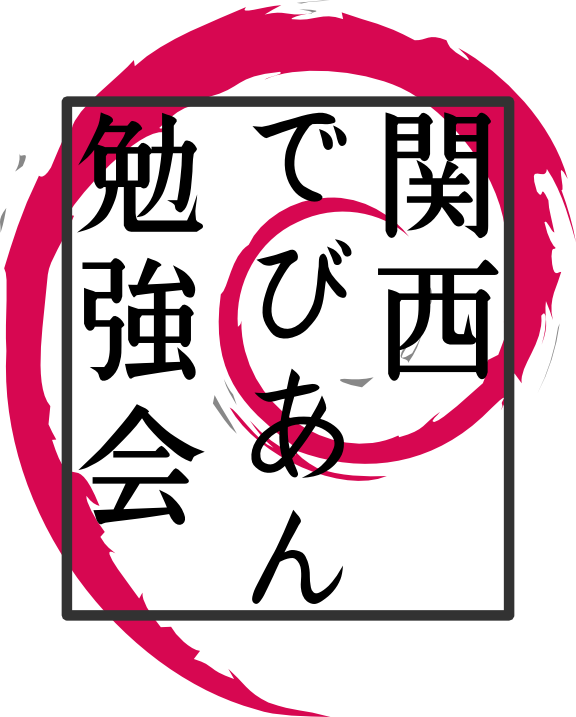
\includegraphics{image200802/kansaidebianlogo.png}
\end{center}

\begin{flushright}
\hfill{}関西 Debian 勉強会担当者 佐々木・倉敷・のがた・かわだ・八津尾 \\
\hfill{}\debmtgyear{}年\debmtgmonth{}月\debmtgdate{}日
\end{flushright}

\thispagestyle{empty}
\end{titlepage}

\dancersection{Introduction}{Debian JP}

\vspace{1em}

 関西Debian勉強会はDebian GNU/Linuxのさまざまなトピック
 (新しいパッケージ、Debian特有の機能の仕組、Debian界隈で起こった出来事、
 などなど)について話し合う会です。

 目的として次の三つを考えています。
 \begin{itemize}
  \item MLや掲示板ではなく、直接顔を合わせる事での情報交換の促進
  \item 定期的に集まれる場所
  \item 資料の作成
 \end{itemize}

 それでは、楽しい一時をお過ごしください。

\newpage

\begin{minipage}[b]{0.2\hsize}
 {\rotatebox{90}{\fontsize{80}{80}
{\gt 関西 Debian 勉強会}}}
\end{minipage}
\begin{minipage}[b]{0.8\hsize}
\hrule
\vspace{2mm}
\hrule
\setcounter{tocdepth}{1}
\tableofcontents
\vspace{2mm}
\hrule
\end{minipage}

\dancersection{最近のDebian関係のイベント報告}{Debian JP}

\subsection{第85回関西Debian勉強会}

85回目の関西Debian勉強会は6月22日(日)に、福島区民センターで行なわれまし
た。

坂本さんによる「Linuxのドライバメンテナになった体験記」と佐々木さんによ
る「Debian での systemd とのつきあい方」のセッション2本立てでした。

systemdは、起動時にresolvconf.serviceとsquid3の循環参照で起動時にタイム
アウト待ちになるという話しを聞くと、Debianで安定して使えるにはもう少し
といったところでしょうか。
とはいえ、現在のsidのGNOME環境ではsystemdでないとすんなり動作しない点も
あり、systemdは避けて通れなくなってきた感じですね。

\subsection{第86回関西Debian勉強会 OSC2014 Kansai@Kyoto}

86回目の関西Debian勉強会は8月2日(土)に、OSC2014 Kansai@Kyotoへの出張開
催しました。

ブースではDebian Jessieの動作マシン展示とTシャツ販売など行ないました。
野方さん作成による新作のTシャツは今年も大変好評でした。

セッションは佐々木さんによる「Debian Project の最近の動向について」と題
した、Jessieに向けて変更点、現在の開発状況のお話しでした。約30名ほどの
方々に参加していただきました。

\subsection{第115回東京エリアDebian勉強会with第2回Debianパッケージング道場}

115回目の東京エリアDebian勉強会は7月19日(土)に株式会社サイバーエージェント
東京オフィス プライムプラザ4F セミナールームBで行なわれました。
今回はDebianパッケージング道場と共催する形での開催となり朝から丸一日
Debian漬けでDebianパッケージを作成する回でした。

\subsection{第116回東京エリアDebian勉強会}

116回目の東京エリアDebian勉強会は8月23日(土)に株式会社スクウェア・エニッ
クス セミナールームで開催されました。

なかおさんによる「Debianでタイルマップサービス作ってみた」のセッションと
もくもくの会で開催されました。

\subsection{Debian Project}

\subsubsection{Debian Day 2014}

8月16日はDebian Dayです。1993年8月16日にIan MurdockさんがDebianを始めて
から今年で21年になりました。今年も世界各国でDebian Dayを祝うイベントが
開催されました。
\footnote{\url{https://wiki.debian.org/DebianDay/2014}}


\subsubsection{Linux kernel version for jessie}

Debian LinuxカーネルチームよりJessieのLinuxカーネルを3.16にするとアナ
ウンスがありました。
\footnote{\url{https://lists.debian.org/debian-devel-announce/2014/07/msg00006.html}}

3.16に対応できないパッケージはこの後削除されていくことになります。また、
3.16はkernel.orgのLongtermブランチではありませんがJessieの通常サポート
期間中はメンテナンスしていけるだろうとのことです。


\subsubsection{Debian Installer Jessie Beta 1 release}

DebianインストーラチームからDebian 8 ``Jessie'' 向けのベータ版インストー
ラがリリースされました。
\footnote{\url{https://lists.debian.org/debian-devel-announce/2014/08/msg00005.html}}

このインストーラからLinux向けinitシステムのデフォルトがsystemdとなって
います。またGNOMEのインストールイメージはxfceでなくGNOMEをインストール
するようになっています。

その他の変更点や最新のインストールイメージはDebianインストーラのニュー
ス
\footnote{\url{https://www.debian.org/devel/debian-installer/News/2014/20140813}}
を参照してください。


\subsubsection{First steps towards source-only uploads}

Ansgar BurchardtさんよりDebianアーカイブへのソースのみのアップロードを
受け付けるようになったとアナウンスがありました。
\footnote{\url{https://lists.debian.org/debian-devel-announce/2014/08/msg00002.html}}

アップロードするには、既にアーカイブに存在していること、新しいバイナリ
を生成しないこと、アーキテクチャ依存を含まないこと、などの条件がありま
すが、まずは第一歩です。

\subsubsection{systemd}

あいかわらずsystemdがdebian-devel@d.oを賑わせているようです。
以前お伝えしたMATE1.8のスレッドもその後systemd絡みで盛り上がりスレッド
が100を越えました。

「How to avoid stealth installation of systemd?」
\footnote{\url{https://lists.debian.org/debian-devel/2014/07/msg00010.html}}

アップグレードしたらsystemdがインストールされて電源ボタンが効かなくなっ
たんだけど、から始まってあっというまにフレーム化。

「systemd now appears to be only possible init system in testing」
\footnote{\url{https://lists.debian.org/debian-devel/2014/07/msg00839.html}}

こちらも似たような感じで、testingにアップグレードしたんだけど
libpam-systemdがsystemd-sysvにdependしてるからsysytemd一択なんだけど、
libpam-systemd取り除いてみたらいろいろ動かないんだけど、から始まって
...。


\subsubsection{RFS: ircii/20131230-1 [NMU]}

よくあるパッケージをNMUしたいからRFSしてくださいということなんですが、
内容をよくみてみるとNew Upstream Releaseの対応で、しかもこのパッケージ
は既にOrphanされていたという。そして何故かUpstream Authorが以前のパッケー
ジメンテナに変わっているというもうなんだかよくわからない内容。

詳しくは\debianbug{756034}をどうぞ。


\subsubsection{DebConf14}

今年のDebian Conference 2014
\footnote{\url{http://debconf14.debconf.org/}}
がアメリカのオレゴン州ポートランドで8/23(土)〜8/31(日)の間開催されてい
ます。

毎年DebConfで色々なことが決まり進んでいくので、今年のDebConfの動向にも
注目です。

セッションの内容はライブ中継されます。また後日、動画とスライドが公開さ
れます。セッションスケジュール
\footnote{\url{https://summit.debconf.org/debconf14/}}
を見て気になるものがあればチェックしてみてはいかがでしょうか。

いくつか紹介します。

\begin{itemize}

\item 2014-08-25 10:00「Meet the Technical Committee」
  \footnote{\url{https://summit.debconf.org/debconf14/meeting/58/meet-the-technical-committee/}}

\item 2014-08-26 13:30「Quit logging! (or, data minimization in Debian)」
  \footnote{\url{https://summit.debconf.org/debconf14/meeting/70/quit-logging-or-data-minimization-in-debian/}}

\item 2014-08-26 14:30「Debian Long Term Support」
  \footnote{\url{https://summit.debconf.org/debconf14/meeting/92/debian-long-term-support/}}

\item 2014-08-26 16:00「Removing obsolete packages for fun and profit」
  \footnote{\url{https://summit.debconf.org/debconf14/meeting/109/removing-obsolete-packages-for-fun-and-profit/}}

\item 2014-08-28 13:30「Validation and Continuous Integration BoF」
  \footnote{\url{https://summit.debconf.org/debconf14/meeting/22/validation-and-continuous-integration-bof/}}

\item 2014-08-28 13:30「New Network Interface Manager for Debian: ifupdown2」
  \footnote{\url{https://summit.debconf.org/debconf14/meeting/6/new-network-interface-manager-for-debian-ifupdown2/}}

\item 2014-08-28 16:00「ACC for abi breaks」
  \footnote{\url{https://summit.debconf.org/debconf14/meeting/62/acc-for-abi-breaks/}}

\item 2014-08-28 16:00「A glimpse into a systemd future」
  \footnote{\url{https://summit.debconf.org/debconf14/meeting/5/a-glimpse-into-a-systemd-future/}}

\item 2014-08-28 19:00「What's new in the Linux kernel」
  \footnote{\url{https://summit.debconf.org/debconf14/meeting/90/whats-new-in-the-linux-kernel/}}

\item 2014-08-29 11:00「debdry - Debian Don't Repeat Yourself」
  \footnote{\url{https://summit.debconf.org/debconf14/meeting/25/debdry-debian-dont-repeat-yourself/}}

\end{itemize}


\dancersection{事前課題}{Debian JP}

今回の課題は以下の通りです。
\begin{screen}
  \begin{enumerate}

  \item %
    もくもくの会で行なう作業、質問などの課題を用意して教えてください。
    (電源とネットワーク(WiMAXなど)はありますが、それ以外の作業に必要な
    環境はご用意ください。)

  \item %
    前回(第85回)の勉強会に参加された方は、前回の作業や課題がその後どう
    なったか結果を教えてください。

  \item %
    LT(ライトニングトーク) 歓迎です。何かお話したい方はタイトルを下さい。

  \end{enumerate}
\end{screen}

参加者の皆さんの解答は以下の通りです:

\begin{prework}{ takata }
  \begin{enumerate}
  \item Docker.ioで クロスツールビルド環境(32ビット・コンテナイメージ)を整備

    参考URL
    \begin{itemize}
    \item 32-bit container on a 64-bit system \#611

      \url{https://github.com/docker/docker/issues/611}
    \item docker で 32bit コンテナイメージを作成する

      \url{http://d.hatena.ne.jp/defiant/20130704/1372947160}
    \end{itemize}
  \item Redmineデータベースの復旧
    wheezyで運用していたときの postgresqlデータベースを jessieの redmine\_{}2.5.2-1に移行。
    \begin{enumerate}
    \item redmine\_{}2.5.2-1は passengerで起動
    \item postgresqlデータベースのリストア
      \begin{commandline}
        $ pg_restore -c -Upostgres --dbname=redmine_default redmine_0.sqlc
      \end{commandline}
      ここで、redmine\_{}0.sqlcは、次の操作で以前に作成したデータベースのバックアップ
      \begin{commandline}
        $ pg_dump -Upostgres --format=c --file=redmine_0.sqlc redmine_default
      \end{commandline}
    \item ownerの変更: redmine -$>$ redmine\_{}default
    \item データベースのマイグレーション(db:migrate)
      \begin{commandline}
        # RAILS_ENV=production rake db:migrate
      \end{commandline}
      このとき、queries\_{}roles, custom\_{}fields\_{}rolesが既に存在するためエラーとなるが、
      テーブルを dropして再試行することでマイグレーションに成功。
      \begin{commandline}
        ii  redmine        2.5.2-1      all          flexible project management web a
        ii  postgresql     9.3+157      all          object-relational SQL database (s
        ii  postgresql-9.3 9.3.4-2      amd64        object-relational SQL database, v
      \end{commandline}
    \end{enumerate}
  \end{enumerate}
\end{prework}

\begin{prework}{ koedoyoshida }
DDTSS翻訳や自分で作成しているソフトのupdate,ボランティアしているOSS関連のイベント作業など。

遅れて参加になると思います。
\end{prework}

\begin{prework}{ かわだてつたろう }
  \begin{enumerate}
  \item 溜っているメールを読む。
  \item gnucacheでかな入力できなかったのはGTK\_{}IM\_{}MODULEがximとなっていたからでした。
    im-configはuim-gtk2.0とuim-gtk3の両方がインストールされていないとGTK\_{}IM\_{}MODULEをuimに設定しない。
  \item ありません。
  \end{enumerate}
\end{prework}

\begin{prework}{ kozo2 }
  \begin{enumerate}
  \item
    \begin{itemize}
    \item [作業] \url{https://bitbucket.org/anekos/iron-maiden-cl}のDebian packageの作成
    \item [質問] 上記作業でわからないことがでたらそれを質問する。

      また\url{https://github.com/spotify/dh-virtualenv}利用経験者がいればそれにまつわる話を聞く。
    \end{itemize}
  \item 前回(第85回)の勉強会に参加していませんでした。
  \item cmakeで.deb作成
  \end{enumerate}
\end{prework}

\begin{prework}{ Mitsutoshi NAKANO $<$bkbin005@rinku.zaq.ne.jp$>$ }
  \begin{enumerate}
  \item a) b)のうちどちらか、または双方。
    \begin{itemize}
    \item [a] tamagoのupstreamの準備

      詳細: \url{http://lists.debian.or.jp/debian-devel/201408/msg00007.html}
    \item [b]Debianのパッケージビルドの方法についての勉強

      詳細: \url{http://lists.debian.or.jp/debian-users/201408/msg00027.html}
    \end{itemize}
  \end{enumerate}
\end{prework}

\begin{prework}{ 坂本 貴史 }
  \begin{enumerate}
  \item 開発中のALSAのドライバを書きます。
  \item 作業や課題とは関係ないのですが、前回受けた質問への回答を、前回分資料に掲載してもらいました。
  \item ネタの用意がありません。
  \end{enumerate}
\end{prework}

\begin{prework}{  清野陽一 }
  \begin{enumerate}
  \item 久しぶりなので最近のDebian界隈の状況を知る。
  \item 不参加
  \item 今のところ無し
  \end{enumerate}
\end{prework}

\begin{prework}{ lurdan }
  \begin{enumerate}
  \item serverspec と e2wm のパッケージ更新
  \item webwml はまだ稼働にこぎつけてないです。これもやらないと……
  \end{enumerate}
\end{prework}

\begin{prework}{ 佐々木洋平 }
  \begin{enumerate}
  \item tDiary の更新
  \item systemd-sysv$<$-$>$sysvinit-core をウロウロしてます。さいきんずっとコレばっか。
  \item 余裕ないです。
  \end{enumerate}
\end{prework}

\begin{prework}{ 川江 }
  \begin{enumerate}
  \item emacsを使って、HTML5のCSS、Javascriptのコードの生成。
  \item 同上(苦戦中)
  \item
  \end{enumerate}
\end{prework}

\dancersection{もくもくの会}{}

\dancersection{今後の予定}{Debian JP}

\subsection{関西Debian勉強会}

次回、第88回関西Debian勉強会は9月28日(日)に福島区民センターで開催予定
です。

\subsection{東京エリアDebian勉強会}

第117回東京エリアDebian勉強会は9月16日(土)に開催予定です。
場所、内容については東京エリアDebian勉強会のウェブサイトを確認してくだ
さい。

%
% 冊子にするために、4の倍数にする必要がある。
% そのための調整
%% \dancersection{メモ}{}
%% \mbox{}\newpage
%% \mbox{}\newpage
%% \mbox{}\newpage

\printindex
%\cleartooddpage

 \begin{minipage}[b]{0.2\hsize}
  \rotatebox{90}{\fontsize{80}{80} {\gt 関西 Debian 勉強会} }
 \end{minipage}
 \begin{minipage}[b]{0.8\hsize}

 \vspace*{15cm}
 \rule{\hsize}{1mm}
 \vspace{2mm}
 
\includegraphics[width=2cm]{image200502/openlogo-nd.eps}
 \noindent \Large \bfseries{Debian 勉強会資料}\\ \\
 \noindent \normalfont \debmtgyear{}年\debmtgmonth{}月\debmtgdate{}日 \hspace{5mm}  初版第1刷発行\\
 \noindent \normalfont 関西 Debian 勉強会 (編集・印刷・発行)\\
 \rule{\hsize}{1mm}
 \end{minipage}

\end{document}
